\begin{apendicesenv}

\partapendices

\chapter{Primeiro Apêndice}

Esse apêndice diz respeito aos códigos feitos na plataforma Scilab.

\section{Módulo Principal}
\label{sec:moduloprincipal}
\begin{lstlisting} 
function DA2 = DA2(som)
	exec get_mono_signal.sci;
	exec get_fourier_transform.sci;
	exec get_equalization_signal.sci;
	exec correlate_with_notes.sci;
	exec correlate_with_chords.sci;
	exec interpret_correlation.sci;

	//Load notes in constants variables
	exec load_notes_constants.sci;

	//Load chords in constants variables
	exec load_chords_constants.sci;

	//Get one dimensional array of signal 
	som = get_mono_signal(som);

	//Get array with slots that are frequencies 
	respfreq = get_fourier_transform(som);
	scf(1); 
	plot(respfreq, '-o');
	xtitle('Resposta em Frequencia', 'Frequencia (Hz)', 'Resposta');
	mtlb_axis([1, 800, 0, 0.7]);

	//Get signal equalizated with maximum is 1
	rfeq = get_equalization_signal(respfreq);

	//Correlate frequencies with array of notes
	scf(2);
	S1 = correlate_with_notes(rfeq);
	bar(S1);
	a=gca();
	notas = ["do" "do#" "re" "re#" "mi" "fa" "fa#" ...
	"sol" "sol#" "la" "la#" "si"]
	notas_slot = [1:12]
	newTicks= a.x_ticks;
	newTicks(2)= notas_slot;
	newTicks(3)= notas;
	a.x_ticks=newTicks;

	//Correlate frequencies with array of chords
	scf(3);
	S2 = correlate_with_chords(S1);
	bar(S2);
	a=gca();
	notas = ["CM" "Cm" "Caum" "Cdim" "C#M" "C#m" "C#aum" "C#dim" ...
	"DM" "Dm" "Daum" "Ddim" ... 
	"D#M" "D#m" "D#aum" "D#dim" ... 
	"EM" "Em" "Eaum" "Edim" ... 
	"FM" "Fm" "Faum" "Fdim" ... 
	"F#M" "F#m" "F#aum" "F#dim" ...
	"GM" "Gm" "Gaum" "Gdim" ...
	"G#M" "G#m" "G#aum" "G#dim" ...
	"AM" "Am" "Aaum" "Adim" ... 
	"A#M" "A#m" "A#aum" "A#dim" ... 
	"BM" "Bm" "Baum" "Bdim"]
	notas_slot = [1:48]
	newTicks= a.x_ticks;
	newTicks(2)= notas_slot;
	newTicks(3)= notas;
	a.x_ticks=newTicks;

	//Get the chord inferred
	ACORDETOC = interpret_correlation(S2);

	DA2 = ACORDETOC;
endfunction
\end{lstlisting}

\section{Módulo de Monoficação do Sinal de Áudio}
\label{sec:modulomonoficacao}
\begin{lstlisting} 
function som = get_mono_signal(som)
	//MONO
	som = som(1:length(som));
	som = som/max(som);
endfunction
\end{lstlisting}

\section{Módulo da Transformada de Fourier}
\label{sec:modulotransformadafourier}
\begin{lstlisting} 
function respfreq = get_fourier_transform(som)
    //--------------------------
    //TRANSFORMADA DE FOURIER
    //tx amostragem
    fs = 44100; 
     //vetor das frequencias disponiveis no som
    f = (0:length(som)-1)*fs/length(som);
    //vetor das frequencias propriamente ditas
    freq = f(1:round(length(f)/2)); 
    //transformada de fourier criando vetor respostas
    SOM = abs(fft(som));
    //normalizacao do vetor das respostas 
    SOM = SOM/max(SOM); 
    //vetor das respostas propriamente ditas
    SOM = SOM(1:round(length(f)/2)); 
    //Transformando as respectivas frequencias em slots
    //variavel auxiliar de contagem dos slots do novo 
    //vetor resposta-frequencia
    l = 1; 
    //variavel auxiliar de contagem das respostas 
    //numa mesma faixa de frequencia
    j = 0; 
    //variavel auxiliar de contagem dos slots do vetor resposta
    i = 1; 
    SOMA = 0; 
    while (i<length(freq))//laco da acoplacao
    	//se as frequencias arrendondadas vizinhas forem iguais...
        if (round(freq(i)) == round(freq(i+1)))
        	//soma das respostas das frequencias parecidas
            SOMA = SOM(i+1) + SOMA;
            //contagem de frequencias parecidas achadas
            j = j + 1;
        else
        	//incersao da media das frequencias parecidas no vetor 
            respfreq(l) = SOMA/(j+1);
            //zerar a contagem das frequencias parecidas 
            //para o proximo conjunto de sequencias
            j = 0;
            SOMA = SOM(i+1);//comecando um novo conjunto de sequencias
            l = l+1;//proximo slot do respfreq
        end
        i = i+1;//proximo slot do vetor SOM   
    end
    //fim do laco e zerando os contadores usados
    l = 0; j = 0; i = 0;
    //--------------------------
endfunction
\end{lstlisting}

\section{Módulo de Equalização do Sinal}
\label{sec:moduloequalizacao}
\begin{lstlisting} 
function rfeq = get_equalization_signal(respfreq)
	//EQUALIZACAO
	x = gsort(respfreq);
	x = x(length(respfreq)-3);
	a = (max(respfreq)-min(respfreq))/x;
	b = max(respfreq)-a*x;
	rfeq = (respfreq-b)/a;
endfunction
\end{lstlisting}

\section{Módulo de Correlação de Notas}
\label{sec:modulocorrelacaonotas}
\begin{lstlisting} 
function S1 = correlate_with_notes(rfeq)

	exec correlation.sci;

	i = 1; //contador para andar ao longo do vetor

	while (i <= 12)
	     correlacao = coeffcorr(rfeq,notas(i,:));
	     S1(i) = correlacao;    
	    //S1(i) = exp(-(norm(rfeq - notas(i,:))*b));
	    i = i + 1;
	end

endfunction
\end{lstlisting}

\section{Módulo de Correlação}
\label{sec:modulocorrelacao}
\begin{lstlisting} 
function [c]=coeffcorr(X,Y)
	// first check consistency of data, return NAN in case of problem
	 [lX,cX]=size(X);
	 if (lX == 1)
	 	X=X';
	 sX=cX;
	 elseif (cX==1)
	 	sX=lX;
	 else
	 	c=%nan;
	 return
	 end
	 [lY,cY]=size(Y);
	 if (lY == 1)
	 	Y=Y';
	 sY=cY;
	 elseif (cY==1)
	 	sY=lY;
	 else
		 c=%nan;
	 return;
	 end
	 if (sX ~= sY)
	 	c=%nan;
	 return;
	 end
	 // here begins the actual computation
	 X=X-mean(X);
	 Y=Y-mean(Y);
	 c=X'*Y;
	 if (c==0)
	 return;
	 else
	 	c=c/(norm(X)*norm(Y));
	 end
 endfunction
\end{lstlisting}

\section{Módulo de Correlação de Acordes}
\label{sec:modulocorrelacaoacordes}
\begin{lstlisting} 
function S2 = correlate_with_chords(S1)
	exec correlation.sci;
	i = 1; //contador para andar ao longo do vetor
	while (i <= 48)
	     correlacao = coeffcorr(S1,BD(:,i)');
	     S2(i) = sqrt(correlacao^2);    
	    i = i + 1;
	end
endfunction
\end{lstlisting}

\section{Módulo de Interpretação de Correlação dos Acordes}
\label{sec:modulocointerpretacao}
\begin{lstlisting} 
function ACORDETOC = interpret_correlation(S2)

acordetoc = find(S2==max(S2));

if (length(acordetoc) > 1)
	acordetoc = acordetoc(1);
end

//DECODIFICADOR

if (acordetoc == 1)
    ACORDETOC = 'CM';
end
if (acordetoc == 2)
    ACORDETOC = 'Cm';
end
if (acordetoc == 3)
    ACORDETOC = 'Caum';
end
if (acordetoc == 4)
    ACORDETOC = 'Cdim';
end
if (acordetoc == 5)
    ACORDETOC = 'C#M';
end
if (acordetoc == 6)
    ACORDETOC = 'C#m';
end
if (acordetoc == 7)
    ACORDETOC = 'C#aum';
end
if (acordetoc == 8)
    ACORDETOC = 'C#dim';
end
if (acordetoc == 9)
    ACORDETOC = 'DM';
end
if (acordetoc == 10)
    ACORDETOC = 'Dm';
end
if (acordetoc == 11)
    ACORDETOC = 'Daum';
end
if (acordetoc == 12)
    ACORDETOC = 'Ddim';
end
if (acordetoc == 13)
    ACORDETOC = 'D#M ou EbM';
end
if (acordetoc == 14)
    ACORDETOC = 'D#m ou Ebm';
end
if (acordetoc == 15)
    ACORDETOC = 'D#aum ou Ebaum';
end
if (acordetoc == 16)
    ACORDETOC = 'D#dim ou Ebdim';
end
if (acordetoc == 17)
    ACORDETOC = 'EM';
end
if (acordetoc == 18)
    ACORDETOC = 'Em';
end
if (acordetoc == 19)
    ACORDETOC = 'Eaum';
end
if (acordetoc == 20)
    ACORDETOC = 'Edim';
end
if (acordetoc == 21)
    ACORDETOC = 'FM';
end
if (acordetoc == 22)
    ACORDETOC = 'Fm';
end
if (acordetoc == 23)
    ACORDETOC = 'Faum';
end
if (acordetoc == 24)
    ACORDETOC = 'Fdim';
end
if (acordetoc == 25)
    ACORDETOC = 'F#M';
end
if (acordetoc == 26)
    ACORDETOC = 'F#m';
end
if (acordetoc == 27)
    ACORDETOC = 'F#aum';
end
if (acordetoc == 28)
    ACORDETOC = 'F#dim';
end
if (acordetoc == 29)
    ACORDETOC = 'GM';
end
if (acordetoc == 30)
    ACORDETOC = 'Gm';
end
if (acordetoc == 31)
    ACORDETOC = 'Gaum';
end
if (acordetoc == 32)
    ACORDETOC = 'Gdim';
end
if (acordetoc == 33)
    ACORDETOC = 'G#M ou AbM';
end
if (acordetoc == 34)
    ACORDETOC = 'G#m ou Abm';
end
if (acordetoc == 35)
    ACORDETOC = 'G#aum ou Abaum';
end
if (acordetoc == 36)
    ACORDETOC = 'G#dim ou Abdim';
end
if (acordetoc == 37)
    ACORDETOC = 'AM';
end
if (acordetoc == 38)
    ACORDETOC = 'Am';
end
if (acordetoc == 39)
    ACORDETOC = 'Aaum';
end
if (acordetoc == 40)
    ACORDETOC = 'Adim';
end
if (acordetoc == 41)
    ACORDETOC = 'A#M ou BbM';
end
if (acordetoc == 42)
    ACORDETOC = 'A#m ou Bbm';
end
if (acordetoc == 43)
    ACORDETOC = 'A#aum ou Bbaum';
end
if (acordetoc == 44)
    ACORDETOC = 'A#dim ou Bbdim';
end
if (acordetoc == 45)
    ACORDETOC = 'BM';
end
if (acordetoc == 46)
    ACORDETOC = 'Bm';
end
if (acordetoc == 47)
    ACORDETOC = 'Baum';
end
if (acordetoc == 48)
    ACORDETOC = 'Bdim';
end
 
endfunction
\end{lstlisting}

\section{Módulo de Alocação de Constantes para Notas}
\label{sec:moduloconstantesnotas}
\begin{lstlisting} 
//--------------------------
//NOTAS

notas(12,22050) = 0; //matriz das notas

//ganhos
g1 = 0.01;
g2 = 0.05;
g3 = 0.1;
g4 = 0.4;
g5 = 0.8;
g6 = 1;

//* Linha[0] = Do */
notas(1 + 0,60) = g1;
notas(1 + 0,61) = g2;
notas(1 + 0,62) = g3;
notas(1 + 0,63) = g4;
notas(1 + 0,64) = g5;
notas(1 + 0,65) = g6;
notas(1 + 0,66) = g5;
notas(1 + 0,67) = g4;
notas(1 + 0,68) = g3;
notas(1 + 0,69) = g2;
notas(1 + 0,70) = g1;

notas(1 + 0,126) = g1;
notas(1 + 0,127) = g2;
notas(1 + 0,128) = g3;
notas(1 + 0,129) = g4;
notas(1 + 0,130) = g5;
notas(1 + 0,131) = g6;
notas(1 + 0,132) = g5;
notas(1 + 0,133) = g4;
notas(1 + 0,134) = g3;
notas(1 + 0,135) = g2;
notas(1 + 0,136) = g1;

notas(1 + 0,256) = g1;
notas(1 + 0,257) = g2;
notas(1 + 0,258) = g3;
notas(1 + 0,259) = g4;
notas(1 + 0,260) = g5;
notas(1 + 0,261) = g6;
notas(1 + 0,262) = g5;
notas(1 + 0,263) = g4;
notas(1 + 0,264) = g3;
notas(1 + 0,265) = g2;
notas(1 + 0,266) = g1;

notas(1 + 0,518) = g1;
notas(1 + 0,519) = g2;
notas(1 + 0,520) = g3;
notas(1 + 0,521) = g4;
notas(1 + 0,522) = g5;
notas(1 + 0,523) = g6;
notas(1 + 0,524) = g5;
notas(1 + 0,525) = g4;
notas(1 + 0,526) = g3;
notas(1 + 0,527) = g2;
notas(1 + 0,528) = g1;

notas(1 + 0,1041) = g1;
notas(1 + 0,1042) = g2;
notas(1 + 0,1043) = g3;
notas(1 + 0,1044) = g4;
notas(1 + 0,1045) = g5;
notas(1 + 0,1046) = g6;
notas(1 + 0,1047) = g5;
notas(1 + 0,1048) = g4;
notas(1 + 0,1049) = g3;
notas(1 + 0,1050) = g2;
notas(1 + 0,1051) = g1;

//* Linha[1] = Do# */
notas(1 + 1,64) = g1;
notas(1 + 1,65) = g2;
notas(1 + 1,66) = g3;
notas(1 + 1,67) = g4;
notas(1 + 1,68) = g5;
notas(1 + 1,69) = g6;
notas(1 + 1,70) = g5;
notas(1 + 1,71) = g4;
notas(1 + 1,72) = g3;
notas(1 + 1,73) = g2;
notas(1 + 1,74) = g1;

notas(1 + 1,133) = g1;
notas(1 + 1,134) = g2;
notas(1 + 1,135) = g3;
notas(1 + 1,136) = g4;
notas(1 + 1,137) = g5;
notas(1 + 1,138) = g6;
notas(1 + 1,139) = g5;
notas(1 + 1,140) = g4;
notas(1 + 1,141) = g3;
notas(1 + 1,142) = g2;
notas(1 + 1,143) = g1;

notas(1 + 1,272) = g1;
notas(1 + 1,273) = g2;
notas(1 + 1,274) = g3;
notas(1 + 1,275) = g4;
notas(1 + 1,276) = g5;
notas(1 + 1,277) = g6;
notas(1 + 1,278) = g5;
notas(1 + 1,279) = g4;
notas(1 + 1,280) = g3;
notas(1 + 1,281) = g2;
notas(1 + 1,282) = g1;

notas(1 + 1,549) = g1;
notas(1 + 1,550) = g2;
notas(1 + 1,551) = g3;
notas(1 + 1,552) = g4;
notas(1 + 1,553) = g5;
notas(1 + 1,554) = g6;
notas(1 + 1,555) = g5;
notas(1 + 1,556) = g4;
notas(1 + 1,557) = g3;
notas(1 + 1,558) = g2;
notas(1 + 1,559) = g1;

notas(1 + 1,1104) = g1;
notas(1 + 1,1105) = g2;
notas(1 + 1,1106) = g3;
notas(1 + 1,1107) = g4;
notas(1 + 1,1108) = g5;
notas(1 + 1,1109) = g6;
notas(1 + 1,1110) = g5;
notas(1 + 1,1111) = g4;
notas(1 + 1,1112) = g3;
notas(1 + 1,1113) = g2;
notas(1 + 1,1114) = g1;

//* Linha[2] = Re */
notas(1 + 2,68) = g1;
notas(1 + 2,69) = g2;
notas(1 + 2,70) = g3;
notas(1 + 2,71) = g4;
notas(1 + 2,72) = g5;
notas(1 + 2,73) = g6;
notas(1 + 2,74) = g5;
notas(1 + 2,75) = g4;
notas(1 + 2,76) = g3;
notas(1 + 2,77) = g2;
notas(1 + 2,78) = g1;

notas(1 + 2,142) = g1;
notas(1 + 2,143) = g2;
notas(1 + 2,144) = g3;
notas(1 + 2,145) = g4;
notas(1 + 2,146) = g5;
notas(1 + 2,147) = g6;
notas(1 + 2,148) = g5;
notas(1 + 2,149) = g4;
notas(1 + 2,150) = g3;
notas(1 + 2,151) = g2;
notas(1 + 2,152) = g1;

notas(1 + 2,289) = g1;
notas(1 + 2,290) = g2;
notas(1 + 2,291) = g3;
notas(1 + 2,292) = g4;
notas(1 + 2,293) = g5;
notas(1 + 2,294) = g6;
notas(1 + 2,295) = g5;
notas(1 + 2,296) = g4;
notas(1 + 2,297) = g3;
notas(1 + 2,298) = g2;
notas(1 + 2,299) = g1;

notas(1 + 2,582) = g1;
notas(1 + 2,583) = g2;
notas(1 + 2,584) = g3;
notas(1 + 2,585) = g4;
notas(1 + 2,586) = g5;
notas(1 + 2,587) = g6;
notas(1 + 2,588) = g5;
notas(1 + 2,589) = g4;
notas(1 + 2,590) = g3;
notas(1 + 2,591) = g2;
notas(1 + 2,592) = g1;

notas(1 + 2,1169) = g1;
notas(1 + 2,1170) = g2;
notas(1 + 2,1171) = g3;
notas(1 + 2,1172) = g4;
notas(1 + 2,1173) = g5;
notas(1 + 2,1174) = g6;
notas(1 + 2,1175) = g5;
notas(1 + 2,1176) = g4;
notas(1 + 2,1177) = g3;
notas(1 + 2,1178) = g2;
notas(1 + 2,1179) = g1;

//* Linha[3] = Re# */
notas(1 + 3,73) = g1;
notas(1 + 3,74) = g2;
notas(1 + 3,75) = g3;
notas(1 + 3,76) = g4;
notas(1 + 3,77) = g5;
notas(1 + 3,78) = g6;
notas(1 + 3,79) = g5;
notas(1 + 3,80) = g4;
notas(1 + 3,81) = g3;
notas(1 + 3,82) = g2;
notas(1 + 3,83) = g1;

notas(1 + 3,140) = g1;
notas(1 + 3,141) = g2;
notas(1 + 3,152) = g3;
notas(1 + 3,153) = g4;
notas(1 + 3,154) = g5;
notas(1 + 3,155) = g6;
notas(1 + 3,156) = g5;
notas(1 + 3,157) = g4;
notas(1 + 3,158) = g3;
notas(1 + 3,159) = g2;
notas(1 + 3,160) = g1;

notas(1 + 3,306) = g1;
notas(1 + 3,307) = g2;
notas(1 + 3,308) = g3;
notas(1 + 3,309) = g4;
notas(1 + 3,310) = g5;
notas(1 + 3,311) = g6;
notas(1 + 3,312) = g5;
notas(1 + 3,313) = g4;
notas(1 + 3,314) = g3;
notas(1 + 3,315) = g2;
notas(1 + 3,316) = g1;

notas(1 + 3,617) = g1;
notas(1 + 3,618) = g2;
notas(1 + 3,619) = g3;
notas(1 + 3,620) = g4;
notas(1 + 3,621) = g5;
notas(1 + 3,622) = g6;
notas(1 + 3,623) = g5;
notas(1 + 3,624) = g4;
notas(1 + 3,625) = g3;
notas(1 + 3,626) = g2;
notas(1 + 3,627) = g1;

notas(1 + 3,1240) = g1;
notas(1 + 3,1241) = g2;
notas(1 + 3,1242) = g3;
notas(1 + 3,1243) = g4;
notas(1 + 3,1244) = g5;
notas(1 + 3,1245) = g6;
notas(1 + 3,1246) = g5;
notas(1 + 3,1247) = g4;
notas(1 + 3,1248) = g3;
notas(1 + 3,1249) = g2;
notas(1 + 3,1250) = g1;

//* Linha[4] = Mi */
notas(1 + 4,77) = g1;
notas(1 + 4,78) = g2;
notas(1 + 4,79) = g3;
notas(1 + 4,80) = g4;
notas(1 + 4,81) = g5;
notas(1 + 4,82) = g6;
notas(1 + 4,83) = g5;
notas(1 + 4,84) = g4;
notas(1 + 4,85) = g3;
notas(1 + 4,86) = g2;
notas(1 + 4,87) = g1;

notas(1 + 4,160) = g1;
notas(1 + 4,161) = g2;
notas(1 + 4,162) = g3;
notas(1 + 4,163) = g4;
notas(1 + 4,164) = g5;
notas(1 + 4,165) = g6;
notas(1 + 4,166) = g5;
notas(1 + 4,167) = g4;
notas(1 + 4,168) = g3;
notas(1 + 4,169) = g2;
notas(1 + 4,170) = g1;

notas(1 + 4,325) = g1;
notas(1 + 4,326) = g2;
notas(1 + 4,327) = g3;
notas(1 + 4,328) = g4;
notas(1 + 4,329) = g5;
notas(1 + 4,330) = g6;
notas(1 + 4,331) = g5;
notas(1 + 4,332) = g4;
notas(1 + 4,333) = g3;
notas(1 + 4,334) = g2;
notas(1 + 4,335) = g1;

notas(1 + 4,655) = g1;
notas(1 + 4,656) = g2;
notas(1 + 4,657) = g3;
notas(1 + 4,658) = g4;
notas(1 + 4,659) = g5;
notas(1 + 4,660) = g6;
notas(1 + 4,661) = g5;
notas(1 + 4,662) = g4;
notas(1 + 4,663) = g3;
notas(1 + 4,664) = g2;
notas(1 + 4,665) = g1;

notas(1 + 4,1313) = g1;
notas(1 + 4,1314) = g2;
notas(1 + 4,1315) = g3;
notas(1 + 4,1316) = g4;
notas(1 + 4,1317) = g5;
notas(1 + 4,1318) = g6;
notas(1 + 4,1319) = g5;
notas(1 + 4,1320) = g4;
notas(1 + 4,1321) = g3;
notas(1 + 4,1322) = g2;
notas(1 + 4,1323) = g1;

//* Linha[5] = Fa */
notas(1 + 5,82) = g1;
notas(1 + 5,83) = g2;
notas(1 + 5,84) = g3;
notas(1 + 5,85) = g4;
notas(1 + 5,86) = g5;
notas(1 + 5,87) = g6;
notas(1 + 5,88) = g5;
notas(1 + 5,89) = g4;
notas(1 + 5,90) = g3;
notas(1 + 5,91) = g2;
notas(1 + 5,92) = g1;

notas(1 + 5,170) = g1;
notas(1 + 5,171) = g2;
notas(1 + 5,172) = g3;
notas(1 + 5,173) = g4;
notas(1 + 5,174) = g5;
notas(1 + 5,175) = g6;
notas(1 + 5,176) = g5;
notas(1 + 5,177) = g4;
notas(1 + 5,178) = g3;
notas(1 + 5,189) = g2;
notas(1 + 5,190) = g1;

notas(1 + 5,344) = g1;
notas(1 + 5,345) = g2;
notas(1 + 5,346) = g3;
notas(1 + 5,347) = g4;
notas(1 + 5,348) = g5;
notas(1 + 5,349) = g6;
notas(1 + 5,350) = g5;
notas(1 + 5,351) = g4;
notas(1 + 5,352) = g3;
notas(1 + 5,353) = g2;
notas(1 + 5,354) = g1;

notas(1 + 5,693) = g1;
notas(1 + 5,694) = g2;
notas(1 + 5,695) = g3;
notas(1 + 5,696) = g4;
notas(1 + 5,697) = g5;
notas(1 + 5,698) = g6;
notas(1 + 5,699) = g5;
notas(1 + 5,700) = g4;
notas(1 + 5,701) = g3;
notas(1 + 5,702) = g2;
notas(1 + 5,703) = g1;

notas(1 + 5,1392) = g1;
notas(1 + 5,1393) = g2;
notas(1 + 5,1394) = g3;
notas(1 + 5,1395) = g4;
notas(1 + 5,1396) = g5;
notas(1 + 5,1397) = g6;
notas(1 + 5,1398) = g5;
notas(1 + 5,1399) = g4;
notas(1 + 5,1400) = g3;
notas(1 + 5,1401) = g2;
notas(1 + 5,1402) = g1;

//* Linha[6] = Fa# */
notas(1 + 6,88) = g1;
notas(1 + 6,89) = g2;
notas(1 + 6,90) = g3;
notas(1 + 6,91) = g4;
notas(1 + 6,92) = g5;
notas(1 + 6,93) = g6;
notas(1 + 6,94) = g5;
notas(1 + 6,95) = g4;
notas(1 + 6,96) = g3;
notas(1 + 6,97) = g2;
notas(1 + 6,98) = g1;

notas(1 + 6,180) = g1;
notas(1 + 6,181) = g2;
notas(1 + 6,182) = g3;
notas(1 + 6,183) = g4;
notas(1 + 6,184) = g5;
notas(1 + 6,185) = g6;
notas(1 + 6,186) = g5;
notas(1 + 6,187) = g4;
notas(1 + 6,188) = g3;
notas(1 + 6,189) = g2;
notas(1 + 6,190) = g1;

notas(1 + 6,365) = g1;
notas(1 + 6,366) = g2;
notas(1 + 6,367) = g3;
notas(1 + 6,368) = g4;
notas(1 + 6,369) = g5;
notas(1 + 6,370) = g6;
notas(1 + 6,371) = g5;
notas(1 + 6,372) = g4;
notas(1 + 6,373) = g3;
notas(1 + 6,374) = g2;
notas(1 + 6,375) = g1;

notas(1 + 6,735) = g1;
notas(1 + 6,736) = g2;
notas(1 + 6,737) = g3;
notas(1 + 6,738) = g4;
notas(1 + 6,739) = g5;
notas(1 + 6,740) = g6;
notas(1 + 6,741) = g5;
notas(1 + 6,742) = g4;
notas(1 + 6,743) = g3;
notas(1 + 6,744) = g2;
notas(1 + 6,745) = g1;

notas(1 + 6,1475) = g1;
notas(1 + 6,1476) = g2;
notas(1 + 6,1477) = g3;
notas(1 + 6,1478) = g4;
notas(1 + 6,1479) = g5;
notas(1 + 6,1480) = g6;
notas(1 + 6,1481) = g5;
notas(1 + 6,1482) = g4;
notas(1 + 6,1483) = g3;
notas(1 + 6,1484) = g2;
notas(1 + 6,1485) = g1;

//* Linha[7] = Sol */
notas(1 + 7,93) = g1;
notas(1 + 7,94) = g2;
notas(1 + 7,95) = g3;
notas(1 + 7,96) = g4;
notas(1 + 7,97) = g5;
notas(1 + 7,98) = g6;
notas(1 + 7,99) = g5;
notas(1 + 7,100) = g4;
notas(1 + 7,101) = g3;
notas(1 + 7,102) = g2;
notas(1 + 7,103) = g1;

notas(1 + 7,191) = g1;
notas(1 + 7,192) = g2;
notas(1 + 7,193) = g3;
notas(1 + 7,194) = g4;
notas(1 + 7,195) = g5;
notas(1 + 7,196) = g6;
notas(1 + 7,197) = g5;
notas(1 + 7,198) = g4;
notas(1 + 7,199) = g3;
notas(1 + 7,200) = g2;
notas(1 + 7,201) = g1;

notas(1 + 7,387) = g1;
notas(1 + 7,388) = g2;
notas(1 + 7,389) = g3;
notas(1 + 7,390) = g4;
notas(1 + 7,391) = g5;
notas(1 + 7,392) = g6;
notas(1 + 7,393) = g5;
notas(1 + 7,394) = g4;
notas(1 + 7,395) = g3;
notas(1 + 7,396) = g2;
notas(1 + 7,397) = g1;

notas(1 + 7,779) = g1;
notas(1 + 7,780) = g2;
notas(1 + 7,781) = g3;
notas(1 + 7,782) = g4;
notas(1 + 7,783) = g5;
notas(1 + 7,784) = g6;
notas(1 + 7,785) = g5;
notas(1 + 7,786) = g4;
notas(1 + 7,787) = g3;
notas(1 + 7,788) = g2;
notas(1 + 7,789) = g1;

notas(1 + 7,1563) = g1;
notas(1 + 7,1564) = g2;
notas(1 + 7,1565) = g3;
notas(1 + 7,1566) = g4;
notas(1 + 7,1567) = g5;
notas(1 + 7,1568) = g6;
notas(1 + 7,1569) = g5;
notas(1 + 7,1570) = g4;
notas(1 + 7,1571) = g3;
notas(1 + 7,1572) = g2;
notas(1 + 7,1573) = g1;

//* Linha[8] = Sol# */
notas(1 + 8,101) = g1;
notas(1 + 8,100) = g2;
notas(1 + 8,101) = g3;
notas(1 + 8,102) = g4;
notas(1 + 8,103) = g5;
notas(1 + 8,104) = g6;
notas(1 + 8,105) = g5;
notas(1 + 8,106) = g4;
notas(1 + 8,107) = g3;
notas(1 + 8,108) = g2;
notas(1 + 8,109) = g1;

notas(1 + 8,203) = g1;
notas(1 + 8,204) = g2;
notas(1 + 8,205) = g3;
notas(1 + 8,206) = g4;
notas(1 + 8,207) = g5;
notas(1 + 8,208) = g6;
notas(1 + 8,209) = g5;
notas(1 + 8,210) = g4;
notas(1 + 8,211) = g3;
notas(1 + 8,212) = g2;
notas(1 + 8,213) = g1;

notas(1 + 8,410) = g1;
notas(1 + 8,411) = g2;
notas(1 + 8,412) = g3;
notas(1 + 8,413) = g4;
notas(1 + 8,414) = g5;
notas(1 + 8,415) = g6;
notas(1 + 8,416) = g5;
notas(1 + 8,417) = g4;
notas(1 + 8,418) = g3;
notas(1 + 8,419) = g2;
notas(1 + 8,420) = g1;

notas(1 + 8,825) = g1;
notas(1 + 8,826) = g2;
notas(1 + 8,827) = g3;
notas(1 + 8,828) = g4;
notas(1 + 8,829) = g5;
notas(1 + 8,830) = g6;
notas(1 + 8,831) = g5;
notas(1 + 8,832) = g4;
notas(1 + 8,833) = g3;
notas(1 + 8,834) = g2;
notas(1 + 8,835) = g1;

notas(1 + 8,1656) = g1;
notas(1 + 8,1657) = g2;
notas(1 + 8,1658) = g3;
notas(1 + 8,1659) = g4;
notas(1 + 8,1660) = g5;
notas(1 + 8,1661) = g6;
notas(1 + 8,1662) = g5;
notas(1 + 8,1663) = g4;
notas(1 + 8,1664) = g3;
notas(1 + 8,1665) = g2;
notas(1 + 8,1666) = g1;

//* Linha[9] = La */
notas(1 + 9,105) = g1;
notas(1 + 9,106) = g2;
notas(1 + 9,107) = g3;
notas(1 + 9,108) = g4;
notas(1 + 9,109) = g5;
notas(1 + 9,110) = g6;
notas(1 + 9,111) = g5;
notas(1 + 9,112) = g4;
notas(1 + 9,113) = g3;
notas(1 + 9,114) = g2;
notas(1 + 9,115) = g1;

notas(1 + 9,215) = g1;
notas(1 + 9,216) = g2;
notas(1 + 9,217) = g3;
notas(1 + 9,218) = g4;
notas(1 + 9,219) = g5;
notas(1 + 9,220) = g6;
notas(1 + 9,221) = g5;
notas(1 + 9,222) = g4;
notas(1 + 9,223) = g3;
notas(1 + 9,224) = g2;
notas(1 + 9,225) = g1;

notas(1 + 9,435) = g1;
notas(1 + 9,436) = g2;
notas(1 + 9,437) = g3;
notas(1 + 9,438) = g4;
notas(1 + 9,439) = g5;
notas(1 + 9,440) = g6;
notas(1 + 9,441) = g5;
notas(1 + 9,442) = g4;
notas(1 + 9,443) = g3;
notas(1 + 9,444) = g2;
notas(1 + 9,445) = g1;

notas(1 + 9,875) = g1;
notas(1 + 9,876) = g2;
notas(1 + 9,877) = g3;
notas(1 + 9,878) = g4;
notas(1 + 9,879) = g5;
notas(1 + 9,880) = g6;
notas(1 + 9,881) = g5;
notas(1 + 9,882) = g4;
notas(1 + 9,883) = g3;
notas(1 + 9,884) = g2;
notas(1 + 9,885) = g1;

notas(1 + 9,1755) = g1;
notas(1 + 9,1756) = g2;
notas(1 + 9,1757) = g3;
notas(1 + 9,1758) = g4;
notas(1 + 9,1759) = g5;
notas(1 + 9,1760) = g6;
notas(1 + 9,1761) = g5;
notas(1 + 9,1762) = g4;
notas(1 + 9,1763) = g3;
notas(1 + 9,1764) = g2;
notas(1 + 9,1765) = g1;

//* Linha[10] = La# */
notas(1 + 10,111) = g1;
notas(1 + 10,112) = g2;
notas(1 + 10,113) = g3;
notas(1 + 10,114) = g4;
notas(1 + 10,115) = g5;
notas(1 + 10,116) = g6;
notas(1 + 10,117) = g5;
notas(1 + 10,118) = g4;
notas(1 + 10,119) = g3;
notas(1 + 10,120) = g2;
notas(1 + 10,121) = g1;

notas(1 + 10,228) = g1;
notas(1 + 10,229) = g2;
notas(1 + 10,230) = g3;
notas(1 + 10,231) = g4;
notas(1 + 10,232) = g5;
notas(1 + 10,233) = g6;
notas(1 + 10,234) = g5;
notas(1 + 10,235) = g4;
notas(1 + 10,236) = g3;
notas(1 + 10,237) = g2;
notas(1 + 10,238) = g1;

notas(1 + 10,461) = g1;
notas(1 + 10,462) = g2;
notas(1 + 10,463) = g3;
notas(1 + 10,464) = g4;
notas(1 + 10,465) = g5;
notas(1 + 10,466) = g6;
notas(1 + 10,467) = g5;
notas(1 + 10,468) = g4;
notas(1 + 10,469) = g3;
notas(1 + 10,470) = g2;
notas(1 + 10,471) = g1;

notas(1 + 10,927) = g1;
notas(1 + 10,928) = g2;
notas(1 + 10,929) = g3;
notas(1 + 10,930) = g4;
notas(1 + 10,931) = g5;
notas(1 + 10,932) = g6;
notas(1 + 10,933) = g5;
notas(1 + 10,934) = g4;
notas(1 + 10,935) = g3;
notas(1 + 10,936) = g2;
notas(1 + 10,937) = g1;

notas(1 + 10,1859) = g1;
notas(1 + 10,1860) = g2;
notas(1 + 10,1861) = g3;
notas(1 + 10,1862) = g4;
notas(1 + 10,1863) = g5;
notas(1 + 10,1864) = g6;
notas(1 + 10,1865) = g5;
notas(1 + 10,1866) = g4;
notas(1 + 10,1867) = g3;
notas(1 + 10,1868) = g2;
notas(1 + 10,1869) = g1;

//* Linha[11] = Si */
notas(1 + 11,119) = g1;
notas(1 + 11,120) = g2;
notas(1 + 11,121) = g3;
notas(1 + 11,122) = g4;
notas(1 + 11,123) = g5;
notas(1 + 11,124) = g6;
notas(1 + 11,125) = g5;
notas(1 + 11,126) = g4;
notas(1 + 11,127) = g3;
notas(1 + 11,128) = g2;
notas(1 + 11,129) = g1;

notas(1 + 11,242) = g1;
notas(1 + 11,243) = g2;
notas(1 + 11,244) = g3;
notas(1 + 11,245) = g4;
notas(1 + 11,246) = g5;
notas(1 + 11,247) = g6;
notas(1 + 11,248) = g5;
notas(1 + 11,249) = g4;
notas(1 + 11,250) = g3;
notas(1 + 11,251) = g2;
notas(1 + 11,252) = g1;

notas(1 + 11,489) = g1;
notas(1 + 11,490) = g2;
notas(1 + 11,491) = g3;
notas(1 + 11,492) = g4;
notas(1 + 11,493) = g5;
notas(1 + 11,494) = g6;
notas(1 + 11,495) = g5;
notas(1 + 11,496) = g4;
notas(1 + 11,497) = g3;
notas(1 + 11,498) = g2;
notas(1 + 11,499) = g1;

notas(1 + 11,983) = g1;
notas(1 + 11,984) = g2;
notas(1 + 11,985) = g3;
notas(1 + 11,986) = g4;
notas(1 + 11,987) = g5;
notas(1 + 11,988) = g6;
notas(1 + 11,989) = g5;
notas(1 + 11,990) = g4;
notas(1 + 11,991) = g3;
notas(1 + 11,992) = g2;
notas(1 + 11,993) = g1;

notas(1 + 11,1971) = g1;
notas(1 + 11,1972) = g2;
notas(1 + 11,1973) = g3;
notas(1 + 11,1974) = g4;
notas(1 + 11,1975) = g5;
notas(1 + 11,1976) = g6;
notas(1 + 11,1977) = g5;
notas(1 + 11,1978) = g4;
notas(1 + 11,1979) = g3;
notas(1 + 11,1980) = g2;
notas(1 + 11,1981) = g1;
\end{lstlisting}


\section{Módulo de Alocação de Constantes para Acordes}
\label{sec:moduloconstantesacordes}
\begin{lstlisting} 

//--------------------------
BD(12,48) = 0; // inicializando o banco de dados para acordes
//--------------------------

afin1 = 0; afin2 = 0;

//C
//CM
BD(12,1) = afin1;
BD(1,1) = 1; //baixo
BD(2,1) = afin2;
BD(4,1) = afin1;
BD(5,1) = 1; //terca
BD(6,1) = afin2;
BD(7,1) = afin1;
BD(8,1) = 1; //quinta
BD(9,1) = afin2;
//Cm
BD(12,2) = afin1;
BD(1,2) = 1; //baixo
BD(2,2) = afin2;
BD(3,2) = afin1;
BD(4,2) = 1; //terca
BD(5,2) = afin2;
BD(7,2) = afin1;
BD(8,2) = 1; //quinta
BD(9,2) = afin2;
//Caum
BD(12,3) = afin1;
BD(1,3) = 1; //baixo
BD(2,3) = afin2;
BD(4,3) = afin1;
BD(5,3) = 1; //terca
BD(6,3) = afin2;
BD(8,3) = afin1;
BD(9,3) = 1; //quinta
BD(10,3) = afin2;
//Cdim
BD(12,4) = afin1;
BD(1,4) = 1; //baixo
BD(2,4) = afin2;
BD(3,4) = afin1;
BD(4,4) = 1; //terca
BD(5,4) = afin2;
BD(6,4) = afin1;
BD(7,4) = 1; //quinta
BD(8,4) = afin2;

//C#
//C#M
BD(1,5) = afin1;
BD(2,5) = 1; //baixo
BD(3,5) = afin2;
BD(5,5) = afin1;
BD(6,5) = 1; //terca
BD(7,5) = afin2;
BD(8,5) = afin1;
BD(9,5) = 1; //quinta
BD(10,5) = afin2;
//C#m
BD(1,6) = afin1;
BD(2,6) = 1; //baixo
BD(3,6) = afin2;
BD(4,6) = afin1;
BD(5,6) = 1; //terca
BD(6,6) = afin2;
BD(8,6) = afin1;
BD(9,6) = 1; //quinta
BD(10,6) = afin2;
//C#aum
BD(1,7) = afin1;
BD(2,7) = 1; //baixo
BD(3,7) = afin2;
BD(5,7) = afin1;
BD(6,7) = 1; //terca
BD(7,7) = afin2;
BD(9,7) = afin1;
BD(10,7) = 1; //quinta
BD(11,7) = afin2;
//C#dim
BD(1,8) = afin1;
BD(2,8) = 1; //baixo
BD(3,8) = afin2;
BD(4,8) = afin1;
BD(5,8) = 1; //terca
BD(6,8) = afin2;
BD(7,8) = afin1;
BD(8,8) = 1; //quinta
BD(9,8) = afin2;

//D
//DM
BD(2,9) = afin1;
BD(3,9) = 1; //baixo
BD(4,9) = afin2;
BD(6,9) = afin1;
BD(7,9) = 1; //terca
BD(8,9) = afin2;
BD(9,9) = afin1;
BD(10,9) = 1; //quinta
BD(11,9) = afin2;
//Dm
BD(2,10) = afin1;
BD(3,10) = 1; //baixo
BD(4,10) = afin2;
BD(5,10) = afin1;
BD(6,10) = 1; //terca
BD(7,10) = afin2;
BD(9,10) = afin1;
BD(10,10) = 1; //quinta
BD(11,10) = afin2;
//Daum
BD(2,11) = afin1;
BD(3,11) = 1; //baixo
BD(4,11) = afin2;
BD(6,11) = afin1;
BD(7,11) = 1; //terca
BD(8,11) = afin2;
BD(10,11) = afin1;
BD(11,11) = 1; //quinta
BD(11,11) = afin2;
//Ddim
BD(2,12) = afin1;
BD(3,12) = 1; //baixo
BD(4,12) = afin2;
BD(5,12) = afin1;
BD(6,12) = 1; //terca
BD(7,12) = afin2;
BD(8,12) = afin1;
BD(9,12) = 1; //quinta
BD(10,12) = afin2;

//D#
//D#M
BD(3,13) = afin1;
BD(4,13) = 1; //baixo
BD(5,13) = afin2;
BD(7,13) = afin1;
BD(8,13) = 1; //terca
BD(9,13) = afin2;
BD(10,13) = afin1;
BD(11,13) = 1; //quinta
BD(12,13) = afin2;
//D#m
BD(3,14) = afin1;
BD(4,14) = 1; //baixo
BD(5,14) = afin2;
BD(6,14) = afin1;
BD(7,14) = 1; //terca
BD(8,14) = afin2;
BD(10,14) = afin1;
BD(11,14) = 1; //quinta
BD(12,14) = afin2;
//D#aum
BD(3,15) = afin1;
BD(4,15) = 1; //baixo
BD(5,15) = afin2;
BD(7,15) = afin1;
BD(8,15) = 1; //terca
BD(9,15) = afin2;
BD(11,15) = afin1;
BD(12,15) = 1; //quinta
BD(1,15) = afin2;
//D#dim
BD(3,16) = afin1;
BD(4,16) = 1; //baixo
BD(5,16) = afin2;
BD(6,16) = afin1;
BD(7,16) = 1; //terca
BD(8,16) = afin2;
BD(9,16) = afin1;
BD(10,16) = 1; //quinta
BD(11,16) = afin2;

//E
//EM
BD(4,17) = afin1;
BD(5,17) = 1; //baixo
BD(6,17) = afin2;
BD(8,17) = afin1;
BD(9,17) = 1; //terca
BD(10,17) = afin2;
BD(11,17) = afin1;
BD(12,17) = 1; //quinta
BD(1,17) = afin2;
//Em
BD(4,18) = afin1;
BD(5,18) = 1; //baixo
BD(6,18) = afin2;
BD(7,18) = afin1;
BD(8,18) = 1; //terca
BD(9,18) = afin2;
BD(11,18) = afin1;
BD(12,18) = 1; //quinta
BD(1,18) = afin2;
//Eaum
BD(4,19) = afin1;
BD(5,19) = 1; //baixo
BD(6,19) = afin2;
BD(8,19) = afin1;
BD(9,19) = 1; //terca
BD(10,19) = afin2;
BD(12,19) = afin1;
BD(1,19) = 1; //quinta
BD(2,19) = afin2;
//Edim
BD(4,20) = afin1;
BD(5,20) = 1; //baixo
BD(6,20) = afin2;
BD(7,20) = afin1;
BD(8,20) = 1; //terca
BD(9,20) = afin2;
BD(10,20) = afin1;
BD(11,20) = 1; //quinta
BD(12,20) = afin2;

//F
//FM
BD(5,21) = afin1;
BD(6,21) = 1; //tonica
BD(7,21) = afin2;
BD(9,21) = afin1;
BD(10,21) = 1; //terca
BD(11,21) = afin2;
BD(12,21) = afin1;
BD(1,21) = 1; //quinta
BD(2,21) = afin2;
//Fm
BD(5,22) = afin1;
BD(6,22) = 1;
BD(7,22) = afin2;
BD(8,22) = afin1;
BD(9,22) = 1;
BD(10,22) = afin2;
BD(12,22) = afin1;
BD(1,22) = 1;
BD(2,22) = afin2;
//Faum
BD(5,23) = afin1;
BD(6,23) = 1;
BD(7,23) = afin2;
BD(9,23) = afin1;
BD(10,23) = 1;
BD(11,23) = afin2;
BD(1,23) = afin1;
BD(2,23) = 1;
BD(3,23) = afin2;
//Fdim
BD(5,24) = afin1;
BD(6,24) = 1;
BD(7,24) = afin2;
BD(8,24) = afin1;
BD(9,24) = 1;
BD(10,24) = afin2;
BD(11,24) = afin1;
BD(12,24) = 1;
BD(1,24) = afin2;

//F#
//F#M
BD(6,25) = afin1;
BD(7,25) = 1;
BD(8,25) = afin2;
BD(10,25) = afin1;
BD(11,25) = 1;
BD(12,25) = afin2;
BD(1,25) = afin1;
BD(2,25) = 1;
BD(3,25) = afin2;
//F#m
BD(6,26) = afin1;
BD(7,26) = 1;
BD(8,26) = afin2;
BD(9,26) = afin1;
BD(10,26) = 1;
BD(11,26) = afin2;
BD(1,26) = afin1;
BD(2,26) = 1;
BD(3,26) = afin2;
//F#aum
BD(6,27) = afin1;
BD(7,27) = 1;
BD(8,27) = afin2;
BD(10,27) = afin1;
BD(11,27) = 1;
BD(12,27) = afin2;
BD(2,27) = afin1;
BD(3,27) = 1;
BD(4,27) = afin2;
//F#dim
BD(6,28) = afin1;
BD(7,28) = 1;
BD(8,28) = afin2;
BD(9,28) = afin1;
BD(10,28) = 1;
BD(11,28) = afin2;
BD(12,28) = afin1;
BD(1,28) = 1;
BD(2,28) = afin2;

//G
//GM
BD(7,29) = afin1;
BD(8,29) = 1;
BD(9,29) = afin2;
BD(11,29) = afin1;
BD(12,29) = 1;
BD(1,29) = afin2;
BD(2,29) = afin1;
BD(3,29) = 1;
BD(4,29) = afin2;
//Gm
BD(7,30) = afin1;
BD(8,30) = 1;
BD(9,30) = afin2;
BD(10,30) = afin1;
BD(11,30) = 1;
BD(12,30) = afin2;
BD(2,30) = afin1;
BD(3,30) = 1;
BD(4,30) = afin2;
//Gaum
BD(7,31) = afin1;
BD(8,31) = 1;
BD(9,31) = afin2;
BD(11,31) = afin1;
BD(12,31) = 1;
BD(1,31) = afin2;
BD(3,31) = afin1;
BD(4,31) = 1;
BD(5,31) = afin2;
//Gdim
BD(7,32) = afin1;
BD(8,32) = 1;
BD(9,32) = afin2;
BD(10,32) = afin1;
BD(11,32) = 1;
BD(12,32) = afin2;
BD(1,32) = afin1;
BD(2,32) = 1;
BD(3,32) = afin2;

//G#
//G#M
BD(8,33) = afin1;
BD(9,33) = 1;
BD(10,33) = afin2;
BD(12,33) = afin1;
BD(1,33) = 1;
BD(2,33) = afin2;
BD(3,33) = afin1;
BD(4,33) = 1;
BD(5,33) = afin2;
//G#m
BD(8,34) = afin1;
BD(9,34) = 1;
BD(10,34) = afin2;
BD(11,34) = afin1;
BD(12,34) = 1;
BD(1,34) = afin2;
BD(3,34) = afin1;
BD(4,34) = 1;
BD(5,34) = afin2;
//G#aum
BD(8,35) = afin1;
BD(9,35) = 1;
BD(10,35) = afin2;
BD(12,35) = afin1;
BD(1,35) = 1;
BD(2,35) = afin2;
BD(4,35) = afin1;
BD(5,35) = 1;
BD(6,35) = afin2;
//G#dim
BD(8,36) = afin1;
BD(9,36) = 1;
BD(10,36) = afin2;
BD(11,36) = afin1;
BD(12,36) = 1;
BD(1,36) = afin2;
BD(2,36) = afin1;
BD(3,36) = 1;
BD(4,36) = afin2;

//A
//AM
BD(9,37) = afin1;
BD(10,37) = 1;
BD(11,37) = afin2;
BD(1,37) = afin1;
BD(2,37) = 1;
BD(3,37) = afin2;
BD(4,37) = afin1;
BD(5,37) = 1;
BD(6,37) = afin2;
//Am
BD(9,38) = afin1;
BD(10,38) = 1;
BD(11,38) = afin2;
BD(12,38) = afin1;
BD(1,38) = 1;
BD(2,38) = afin2;
BD(4,38) = afin1;
BD(5,38) = 1;
BD(6,38) = afin2;
//Aaum
BD(9,39) = afin1;
BD(10,39) = 1;
BD(11,39) = afin2;
BD(1,39) = afin1;
BD(2,39) = 1;
BD(3,39) = afin2;
BD(5,39) = afin1;
BD(6,39) = 1;
BD(7,39) = afin2;
//Adim
BD(9,40) = afin1;
BD(10,40) = 1;
BD(11,40) = afin2;
BD(12,40) = afin1;
BD(1,40) = 1;
BD(2,40) = afin2;
BD(3,40) = afin1;
BD(4,40) = 1;
BD(5,40) = afin2;

//A#
//A#M
BD(10,41) = afin1;
BD(11,41) = 1;
BD(12,41) = afin2;
BD(2,41) = afin1;
BD(3,41) = 1;
BD(4,41) = afin2;
BD(5,41) = afin1;
BD(6,41) = 1;
BD(7,41) = afin2;
//A#m
BD(10,42) = afin1;
BD(11,42) = 1;
BD(12,42) = afin2;
BD(1,42) = afin1;
BD(2,42) = 1;
BD(3,42) = afin2;
BD(5,42) = afin1;
BD(6,42) = 1;
BD(7,42) = afin2;
//A#aum
BD(10,43) = afin1;
BD(11,43) = 1;
BD(12,43) = afin2;
BD(2,43) = afin1;
BD(3,43) = 1;
BD(4,43) = afin2;
BD(6,43) = afin1;
BD(7,43) = 1;
BD(8,43) = afin2;
//A#dim
BD(10,44) = afin1;
BD(11,44) = 1;
BD(12,44) = afin2;
BD(1,44) = afin1;
BD(2,44) = 1;
BD(3,44) = afin2;
BD(4,44) = afin1;
BD(5,44) = 1;
BD(6,44) = afin2;

//B
//BM
BD(11,45) = afin1;
BD(12,45) = 1;
BD(1,45) = afin2;
BD(3,45) = afin1;
BD(4,45) = 1;
BD(5,45) = afin2;
BD(6,45) = afin1;
BD(7,45) = 1;
BD(8,45) = afin2;
//Bm
BD(11,46) = afin1;
BD(12,46) = 1;
BD(1,46) = afin2;
BD(2,46) = afin1;
BD(3,46) = 1;
BD(4,46) = afin2;
BD(6,46) = afin1;
BD(7,46) = 1;
BD(8,46) = afin2;
//Baum
BD(11,47) = afin1;
BD(12,47) = 1;
BD(1,47) = afin2;
BD(3,47) = afin1;
BD(4,47) = 1;
BD(5,47) = afin2;
BD(7,47) = afin1;
BD(8,47) = 1;
BD(9,47) = afin2;
//Bdim
BD(11,48) = afin1;
BD(12,48) = 1;
BD(1,48) = afin2;
BD(2,48) = afin1;
BD(3,48) = 1;
BD(4,48) = afin2;
BD(5,48) = afin1;
BD(6,48) = 1;
BD(7,48) = afin2;
\end{lstlisting}

\section{Módulo de Testes em Amostras}
\label{sec:moduloequalizacao}
\begin{lstlisting} 
exec dc.sci;

//Script to tests

//Open the file to write results
file_results = mopen('chords_results.txt','w');

chord = 0;

//Testing combinations of CM
chord_result_1 = DA2(wavread('acordes_teste/CM1.wav'));
chord = chord + 1;
disp(chord)
chord_result_2 = DA2(wavread('acordes_teste/CM2.wav'));
chord = chord + 1;
disp(chord)
chord_result_3 = DA2(wavread('acordes_teste/CM3.wav'));
chord = chord + 1;
disp(chord)
mputl(chord_result_1+';'+chord_result_2+';'+chord_result_3,file_results);
//Testing combinations of Cm
chord_result_1 = DA2(wavread('acordes_teste/Cm1.wav'));
chord = chord + 1;
disp(chord)
chord_result_2 = DA2(wavread('acordes_teste/Cm2.wav'));
chord = chord + 1;
disp(chord)
chord_result_3 = DA2(wavread('acordes_teste/Cm3.wav'));
chord = chord + 1;
disp(chord)
mputl(chord_result_1+';'+chord_result_2+';'+chord_result_3,file_results);
//Testing combinations of Caum
chord_result_1 = DA2(wavread('acordes_teste/Caum1.wav'));
chord = chord + 1;
disp(chord)
chord_result_2 = DA2(wavread('acordes_teste/Caum2.wav'));
chord = chord + 1;
disp(chord)
chord_result_3 = DA2(wavread('acordes_teste/Caum3.wav'));
chord = chord + 1;
disp(chord)
mputl(chord_result_1+';'+chord_result_2+';'+chord_result_3,file_results);
//Testing combinations of Cdim
chord_result_1 = DA2(wavread('acordes_teste/Cdim1.wav'));
chord = chord + 1;
disp(chord)
chord_result_2 = DA2(wavread('acordes_teste/Cdim2.wav'));
chord = chord + 1;
disp(chord)
chord_result_3 = DA2(wavread('acordes_teste/Cdim3.wav'));
chord = chord + 1;
disp(chord)
mputl(chord_result_1+';'+chord_result_2+';'+chord_result_3,file_results);

//Testing combinations of C#M
chord_result_1 = DA2(wavread('acordes_teste/C#M1.wav'));
chord = chord + 1;
disp(chord)
chord_result_2 = DA2(wavread('acordes_teste/C#M2.wav'));
chord = chord + 1;
disp(chord)
chord_result_3 = DA2(wavread('acordes_teste/C#M3.wav'));
chord = chord + 1;
disp(chord)
mputl(chord_result_1+';'+chord_result_2+';'+chord_result_3,file_results);
//Testing combinations of C#m
chord_result_1 = DA2(wavread('acordes_teste/C#m1.wav'));
chord = chord + 1;
disp(chord)
chord_result_2 = DA2(wavread('acordes_teste/C#m2.wav'));
chord = chord + 1;
disp(chord)
chord_result_3 = DA2(wavread('acordes_teste/C#m3.wav'));
chord = chord + 1;
disp(chord)
mputl(chord_result_1+';'+chord_result_2+';'+chord_result_3,file_results);
//Testing combinations of C#aum
chord_result_1 = DA2(wavread('acordes_teste/C#aum1.wav'));
chord = chord + 1;
disp(chord)
chord_result_2 = DA2(wavread('acordes_teste/C#aum2.wav'));
chord = chord + 1;
disp(chord)
chord_result_3 = DA2(wavread('acordes_teste/C#aum3.wav'));
chord = chord + 1;
disp(chord)
mputl(chord_result_1+';'+chord_result_2+';'+chord_result_3,file_results);
//Testing combinations of C#dim
chord_result_1 = DA2(wavread('acordes_teste/C#dim1.wav'));
chord = chord + 1;
disp(chord)
chord_result_2 = DA2(wavread('acordes_teste/C#dim2.wav'));
chord = chord + 1;
disp(chord)
chord_result_3 = DA2(wavread('acordes_teste/C#dim3.wav'));
chord = chord + 1;
disp(chord)
mputl(chord_result_1+';'+chord_result_2+';'+chord_result_3,file_results);

//Testing combinations of DM
chord_result_1 = DA2(wavread('acordes_teste/DM1.wav'));
chord = chord + 1;
disp(chord)
chord_result_2 = DA2(wavread('acordes_teste/DM2.wav'));
chord = chord + 1;
disp(chord)
chord_result_3 = DA2(wavread('acordes_teste/DM3.wav'));
chord = chord + 1;
disp(chord)
mputl(chord_result_1+';'+chord_result_2+';'+chord_result_3,file_results);
//Testing combinations of Dm
chord_result_1 = DA2(wavread('acordes_teste/Dm1.wav'));
chord = chord + 1;
disp(chord)
chord_result_2 = DA2(wavread('acordes_teste/Dm2.wav'));
chord = chord + 1;
disp(chord)
chord_result_3 = DA2(wavread('acordes_teste/Dm3.wav'));
chord = chord + 1;
disp(chord)
mputl(chord_result_1+';'+chord_result_2+';'+chord_result_3,file_results);
//Testing combinations of Daum
chord_result_1 = DA2(wavread('acordes_teste/Daum1.wav'));
chord = chord + 1;
disp(chord)
chord_result_2 = DA2(wavread('acordes_teste/Daum2.wav'));
chord = chord + 1;
disp(chord)
chord_result_3 = DA2(wavread('acordes_teste/Daum3.wav'));
chord = chord + 1;
disp(chord)
mputl(chord_result_1+';'+chord_result_2+';'+chord_result_3,file_results);
//Testing combinations of Ddim
chord_result_1 = DA2(wavread('acordes_teste/Ddim1.wav'));
chord = chord + 1;
disp(chord)
chord_result_2 = DA2(wavread('acordes_teste/Ddim2.wav'));
chord = chord + 1;
disp(chord)
chord_result_3 = DA2(wavread('acordes_teste/Ddim3.wav'));
chord = chord + 1;
disp(chord)
mputl(chord_result_1+';'+chord_result_2+';'+chord_result_3,file_results);

//Testing combinations of D#M
chord_result_1 = DA2(wavread('acordes_teste/D#M1.wav'));
chord = chord + 1;
disp(chord)
chord_result_2 = DA2(wavread('acordes_teste/D#M2.wav'));
chord = chord + 1;
disp(chord)
chord_result_3 = DA2(wavread('acordes_teste/D#M3.wav'));
chord = chord + 1;
disp(chord)
mputl(chord_result_1+';'+chord_result_2+';'+chord_result_3,file_results);
//Testing combinations of D#m
chord_result_1 = DA2(wavread('acordes_teste/D#m1.wav'));
chord = chord + 1;
disp(chord)
chord_result_2 = DA2(wavread('acordes_teste/D#m2.wav'));
chord = chord + 1;
disp(chord)
chord_result_3 = DA2(wavread('acordes_teste/D#m3.wav'));
chord = chord + 1;
disp(chord)
mputl(chord_result_1+';'+chord_result_2+';'+chord_result_3,file_results);
//Testing combinations of D#aum
chord_result_1 = DA2(wavread('acordes_teste/D#aum1.wav'));
chord = chord + 1;
disp(chord)
chord_result_2 = DA2(wavread('acordes_teste/D#aum2.wav'));
chord = chord + 1;
disp(chord)
chord_result_3 = DA2(wavread('acordes_teste/D#aum3.wav'));
chord = chord + 1;
disp(chord)
mputl(chord_result_1+';'+chord_result_2+';'+chord_result_3,file_results);
//Testing combinations of D#dim
chord_result_1 = DA2(wavread('acordes_teste/D#dim1.wav'));
chord = chord + 1;
disp(chord)
chord_result_2 = DA2(wavread('acordes_teste/D#dim2.wav'));
chord = chord + 1;
disp(chord)
chord_result_3 = DA2(wavread('acordes_teste/D#dim3.wav'));
chord = chord + 1;
disp(chord)
mputl(chord_result_1+';'+chord_result_2+';'+chord_result_3,file_results);

//Testing combinations of EM
chord_result_1 = DA2(wavread('acordes_teste/EM1.wav'));
chord = chord + 1;
disp(chord)
chord_result_2 = DA2(wavread('acordes_teste/EM2.wav'));
chord = chord + 1;
disp(chord)
chord_result_3 = DA2(wavread('acordes_teste/EM3.wav'));
chord = chord + 1;
disp(chord)
mputl(chord_result_1+';'+chord_result_2+';'+chord_result_3,file_results);
//Testing combinations of Em
chord_result_1 = DA2(wavread('acordes_teste/Em1.wav'));
chord = chord + 1;
disp(chord)
chord_result_2 = DA2(wavread('acordes_teste/Em2.wav'));
chord = chord + 1;
disp(chord)
chord_result_3 = DA2(wavread('acordes_teste/Em3.wav'));
chord = chord + 1;
disp(chord)
mputl(chord_result_1+';'+chord_result_2+';'+chord_result_3,file_results);
//Testing combinations of Eaum
chord_result_1 = DA2(wavread('acordes_teste/Eaum1.wav'));
chord = chord + 1;
disp(chord)
chord_result_2 = DA2(wavread('acordes_teste/Eaum2.wav'));
chord = chord + 1;
disp(chord)
chord_result_3 = DA2(wavread('acordes_teste/Eaum3.wav'));
chord = chord + 1;
disp(chord)
mputl(chord_result_1+';'+chord_result_2+';'+chord_result_3,file_results);
//Testing combinations of Edim
chord_result_1 = DA2(wavread('acordes_teste/Edim1.wav'));
chord = chord + 1;
disp(chord)
chord_result_2 = DA2(wavread('acordes_teste/Edim2.wav'));
chord = chord + 1;
disp(chord)
chord_result_3 = DA2(wavread('acordes_teste/Edim3.wav'));
chord = chord + 1;
disp(chord)
mputl(chord_result_1+';'+chord_result_2+';'+chord_result_3,file_results);

//Testing combinations of FM
chord_result_1 = DA2(wavread('acordes_teste/FM1.wav'));
chord = chord + 1;
disp(chord)
chord_result_2 = DA2(wavread('acordes_teste/FM2.wav'));
chord = chord + 1;
disp(chord)
chord_result_3 = DA2(wavread('acordes_teste/FM3.wav'));
chord = chord + 1;
disp(chord)
mputl(chord_result_1+';'+chord_result_2+';'+chord_result_3,file_results);
//Testing combinations of Fm
chord_result_1 = DA2(wavread('acordes_teste/Fm1.wav'));
chord = chord + 1;
disp(chord)
chord_result_2 = DA2(wavread('acordes_teste/Fm2.wav'));
chord = chord + 1;
disp(chord)
chord_result_3 = DA2(wavread('acordes_teste/Fm3.wav'));
chord = chord + 1;
disp(chord)
mputl(chord_result_1+';'+chord_result_2+';'+chord_result_3,file_results);
//Testing combinations of Faum
chord_result_1 = DA2(wavread('acordes_teste/Faum1.wav'));
chord = chord + 1;
disp(chord)
chord_result_2 = DA2(wavread('acordes_teste/Faum2.wav'));
chord = chord + 1;
disp(chord)
chord_result_3 = DA2(wavread('acordes_teste/Faum3.wav'));
chord = chord + 1;
disp(chord)
mputl(chord_result_1+';'+chord_result_2+';'+chord_result_3,file_results);
//Testing combinations of Fdim
chord_result_1 = DA2(wavread('acordes_teste/Fdim1.wav'));
chord = chord + 1;
disp(chord)
chord_result_2 = DA2(wavread('acordes_teste/Fdim2.wav'));
chord = chord + 1;
disp(chord)
chord_result_3 = DA2(wavread('acordes_teste/Fdim3.wav'));
chord = chord + 1;
disp(chord)
mputl(chord_result_1+';'+chord_result_2+';'+chord_result_3,file_results);

//Testing combinations of F#M
chord_result_1 = DA2(wavread('acordes_teste/F#M1.wav'));
chord = chord + 1;
disp(chord)
chord_result_2 = DA2(wavread('acordes_teste/F#M2.wav'));
chord = chord + 1;
disp(chord)
chord_result_3 = DA2(wavread('acordes_teste/F#M3.wav'));
chord = chord + 1;
disp(chord)
mputl(chord_result_1+';'+chord_result_2+';'+chord_result_3,file_results);
//Testing combinations of F#m
chord_result_1 = DA2(wavread('acordes_teste/F#m1.wav'));
chord = chord + 1;
disp(chord)
chord_result_2 = DA2(wavread('acordes_teste/F#m2.wav'));
chord = chord + 1;
disp(chord)
chord_result_3 = DA2(wavread('acordes_teste/F#m3.wav'));
chord = chord + 1;
disp(chord)
mputl(chord_result_1+';'+chord_result_2+';'+chord_result_3,file_results);
//Testing combinations of F#aum
chord_result_1 = DA2(wavread('acordes_teste/F#aum1.wav'));
chord = chord + 1;
disp(chord)
chord_result_2 = DA2(wavread('acordes_teste/F#aum2.wav'));
chord = chord + 1;
disp(chord)
chord_result_3 = DA2(wavread('acordes_teste/F#aum3.wav'));
chord = chord + 1;
disp(chord)
mputl(chord_result_1+';'+chord_result_2+';'+chord_result_3,file_results);
//Testing combinations of F#dim
chord_result_1 = DA2(wavread('acordes_teste/F#dim1.wav'));
chord = chord + 1;
disp(chord)
chord_result_2 = DA2(wavread('acordes_teste/F#dim2.wav'));
chord = chord + 1;
disp(chord)
chord_result_3 = DA2(wavread('acordes_teste/F#dim3.wav'));
chord = chord + 1;
disp(chord)
mputl(chord_result_1+';'+chord_result_2+';'+chord_result_3,file_results);

//Testing combinations of GM
chord_result_1 = DA2(wavread('acordes_teste/GM1.wav'));
chord = chord + 1;
disp(chord)
chord_result_2 = DA2(wavread('acordes_teste/GM2.wav'));
chord = chord + 1;
disp(chord)
chord_result_3 = DA2(wavread('acordes_teste/GM3.wav'));
chord = chord + 1;
disp(chord)
mputl(chord_result_1+';'+chord_result_2+';'+chord_result_3,file_results);
//Testing combinations of Gm
chord_result_1 = DA2(wavread('acordes_teste/Gm1.wav'));
chord = chord + 1;
disp(chord)
chord_result_2 = DA2(wavread('acordes_teste/Gm2.wav'));
chord = chord + 1;
disp(chord)
chord_result_3 = DA2(wavread('acordes_teste/Gm3.wav'));
chord = chord + 1;
disp(chord)
mputl(chord_result_1+';'+chord_result_2+';'+chord_result_3,file_results);
//Testing combinations of Gaum
chord_result_1 = DA2(wavread('acordes_teste/Gaum1.wav'));
chord = chord + 1;
disp(chord)
chord_result_2 = DA2(wavread('acordes_teste/Gaum2.wav'));
chord = chord + 1;
disp(chord)
chord_result_3 = DA2(wavread('acordes_teste/Gaum3.wav'));
chord = chord + 1;
disp(chord)
mputl(chord_result_1+';'+chord_result_2+';'+chord_result_3,file_results);
//Testing combinations of Gdim
chord_result_1 = DA2(wavread('acordes_teste/Gdim1.wav'));
chord = chord + 1;
disp(chord)
chord_result_2 = DA2(wavread('acordes_teste/Gdim2.wav'));
chord = chord + 1;
disp(chord)
chord_result_3 = DA2(wavread('acordes_teste/Gdim3.wav'));
chord = chord + 1;
disp(chord)
mputl(chord_result_1+';'+chord_result_2+';'+chord_result_3,file_results);

//Testing combinations of G#M
chord_result_1 = DA2(wavread('acordes_teste/G#M1.wav'));
chord = chord + 1;
disp(chord)
chord_result_2 = DA2(wavread('acordes_teste/G#M2.wav'));
chord = chord + 1;
disp(chord)
chord_result_3 = DA2(wavread('acordes_teste/G#M3.wav'));
chord = chord + 1;
disp(chord)
mputl(chord_result_1+';'+chord_result_2+';'+chord_result_3,file_results);
//Testing combinations of G#m
chord_result_1 = DA2(wavread('acordes_teste/G#m1.wav'));
chord = chord + 1;
disp(chord)
chord_result_2 = DA2(wavread('acordes_teste/G#m2.wav'));
chord = chord + 1;
disp(chord)
chord_result_3 = DA2(wavread('acordes_teste/G#m3.wav'));
chord = chord + 1;
disp(chord)
mputl(chord_result_1+';'+chord_result_2+';'+chord_result_3,file_results);
//Testing combinations of G#aum
chord_result_1 = DA2(wavread('acordes_teste/G#aum1.wav'));
chord = chord + 1;
disp(chord)
chord_result_2 = DA2(wavread('acordes_teste/G#aum2.wav'));
chord = chord + 1;
disp(chord)
chord_result_3 = DA2(wavread('acordes_teste/G#aum3.wav'));
chord = chord + 1;
disp(chord)
mputl(chord_result_1+';'+chord_result_2+';'+chord_result_3,file_results);
//Testing combinations of G#dim
chord_result_1 = DA2(wavread('acordes_teste/G#dim1.wav'));
chord = chord + 1;
disp(chord)
chord_result_2 = DA2(wavread('acordes_teste/G#dim2.wav'));
chord = chord + 1;
disp(chord)
chord_result_3 = DA2(wavread('acordes_teste/G#dim3.wav'));
chord = chord + 1;
disp(chord)
mputl(chord_result_1+';'+chord_result_2+';'+chord_result_3,file_results);

//Testing combinations of AM
chord_result_1 = DA2(wavread('acordes_teste/AM1.wav'));
chord = chord + 1;
disp(chord)
chord_result_2 = DA2(wavread('acordes_teste/AM2.wav'));
chord = chord + 1;
disp(chord)
chord_result_3 = DA2(wavread('acordes_teste/AM3.wav'));
chord = chord + 1;
disp(chord)
mputl(chord_result_1+';'+chord_result_2+';'+chord_result_3,file_results);
//Testing combinations of Am
chord_result_1 = DA2(wavread('acordes_teste/Am1.wav'));
chord = chord + 1;
disp(chord)
chord_result_2 = DA2(wavread('acordes_teste/Am2.wav'));
chord = chord + 1;
disp(chord)
chord_result_3 = DA2(wavread('acordes_teste/Am3.wav'));
chord = chord + 1;
disp(chord)
mputl(chord_result_1+';'+chord_result_2+';'+chord_result_3,file_results);
//Testing combinations of Aaum
chord_result_1 = DA2(wavread('acordes_teste/Aaum1.wav'));
chord = chord + 1;
disp(chord)
chord_result_2 = DA2(wavread('acordes_teste/Aaum2.wav'));
chord = chord + 1;
disp(chord)
chord_result_3 = DA2(wavread('acordes_teste/Aaum3.wav'));
chord = chord + 1;
disp(chord)
mputl(chord_result_1+';'+chord_result_2+';'+chord_result_3,file_results);
//Testing combinations of Adim
chord_result_1 = DA2(wavread('acordes_teste/Adim1.wav'));
chord = chord + 1;
disp(chord)
chord_result_2 = DA2(wavread('acordes_teste/Adim2.wav'));
chord = chord + 1;
disp(chord)
chord_result_3 = DA2(wavread('acordes_teste/Adim3.wav'));
chord = chord + 1;
disp(chord)
mputl(chord_result_1+';'+chord_result_2+';'+chord_result_3,file_results);

//Testing combinations of A#M
chord_result_1 = DA2(wavread('acordes_teste/A#M1.wav'));
chord = chord + 1;
disp(chord)
chord_result_2 = DA2(wavread('acordes_teste/A#M2.wav'));
chord = chord + 1;
disp(chord)
chord_result_3 = DA2(wavread('acordes_teste/A#M3.wav'));
chord = chord + 1;
disp(chord)
mputl(chord_result_1+';'+chord_result_2+';'+chord_result_3,file_results);
//Testing combinations of A#m
chord_result_1 = DA2(wavread('acordes_teste/A#m1.wav'));
chord = chord + 1;
disp(chord)
chord_result_2 = DA2(wavread('acordes_teste/A#m2.wav'));
chord = chord + 1;
disp(chord)
chord_result_3 = DA2(wavread('acordes_teste/A#m3.wav'));
chord = chord + 1;
disp(chord)
mputl(chord_result_1+';'+chord_result_2+';'+chord_result_3,file_results);
//Testing combinations of A#aum
chord_result_1 = DA2(wavread('acordes_teste/A#aum1.wav'));
chord = chord + 1;
disp(chord)
chord_result_2 = DA2(wavread('acordes_teste/A#aum2.wav'));
chord = chord + 1;
disp(chord)
chord_result_3 = DA2(wavread('acordes_teste/A#aum3.wav'));
chord = chord + 1;
disp(chord)
mputl(chord_result_1+';'+chord_result_2+';'+chord_result_3,file_results);
//Testing combinations of A#dim
chord_result_1 = DA2(wavread('acordes_teste/A#dim1.wav'));
chord = chord + 1;
disp(chord)
chord_result_2 = DA2(wavread('acordes_teste/A#dim2.wav'));
chord = chord + 1;
disp(chord)
chord_result_3 = DA2(wavread('acordes_teste/A#dim3.wav'));
chord = chord + 1;
disp(chord)
mputl(chord_result_1+';'+chord_result_2+';'+chord_result_3,file_results);

//Testing combinations of BM
chord_result_1 = DA2(wavread('acordes_teste/BM1.wav'));
chord = chord + 1;
disp(chord)
chord_result_2 = DA2(wavread('acordes_teste/BM2.wav'));
chord = chord + 1;
disp(chord)
chord_result_3 = DA2(wavread('acordes_teste/BM3.wav'));
chord = chord + 1;
disp(chord)
mputl(chord_result_1+';'+chord_result_2+';'+chord_result_3,file_results);
//Testing combinations of Bm
chord_result_1 = DA2(wavread('acordes_teste/Bm1.wav'));
chord = chord + 1;
disp(chord)
chord_result_2 = DA2(wavread('acordes_teste/Bm2.wav'));
chord = chord + 1;
disp(chord)
chord_result_3 = DA2(wavread('acordes_teste/Bm3.wav'));
chord = chord + 1;
disp(chord)
mputl(chord_result_1+';'+chord_result_2+';'+chord_result_3,file_results);
//Testing combinations of Baum
chord_result_1 = DA2(wavread('acordes_teste/Baum1.wav'));
chord = chord + 1;
disp(chord)
chord_result_2 = DA2(wavread('acordes_teste/Baum2.wav'));
chord = chord + 1;
disp(chord)
chord_result_3 = DA2(wavread('acordes_teste/Baum3.wav'));
chord = chord + 1;
disp(chord)
mputl(chord_result_1+';'+chord_result_2+';'+chord_result_3,file_results);
//Testing combinations of Bdim
chord_result_1 = DA2(wavread('acordes_teste/Bdim1.wav'));
chord = chord + 1;
disp(chord)
chord_result_2 = DA2(wavread('acordes_teste/Bdim2.wav'));
chord = chord + 1;
disp(chord)
chord_result_3 = DA2(wavread('acordes_teste/Bdim3.wav'));
chord = chord + 1;
disp(chord)
mputl(chord_result_1+';'+chord_result_2+';'+chord_result_3,file_results);

mclose(file_results);
\end{lstlisting}

\end{apendicesenv}

\section{Cronograma para Próximas Atividades}
\label{sec:cronograma}
\begin{figure}[h]
	\centering
		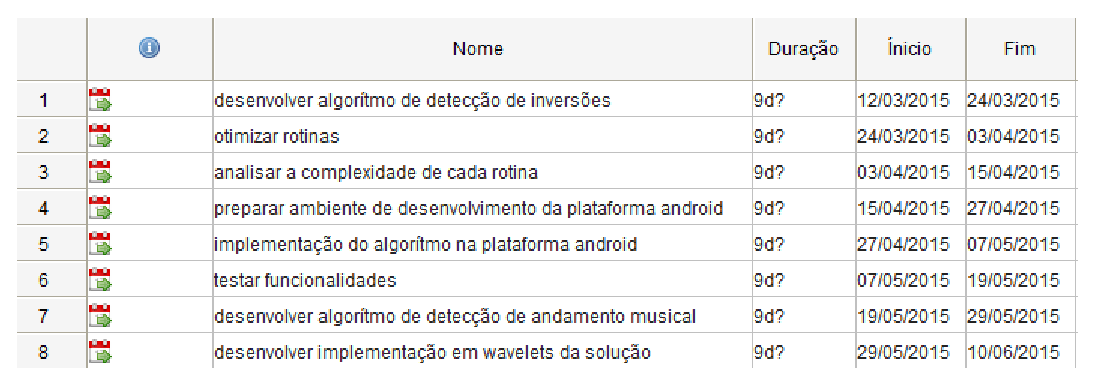
\includegraphics[keepaspectratio=true,scale=0.9]{figuras/cronograma.eps}
	\caption{Cronogroma para Trabalho de Conclusão de Curso 2}
\end{figure}